\documentclass[12pt,a4paper]{article}
\usepackage[utf8]{inputenc}
\usepackage{ngerman}
\usepackage{amsmath}
\usepackage{amsfonts}
\usepackage{amssymb}
\usepackage{graphicx}
\usepackage{color}
\usepackage{enumerate}
\usepackage{lineno}
\usepackage{listings} 
\definecolor{lightgrey}{rgb}{0.90,0.90,0.90}
\lstset{language=Java, backgroundcolor=\color{lightgrey},  numbersep=5pt, tabsize=3}

\setlength{\parindent}{0em}
\setlength{\parskip}{0.5em}

\title{Lösungsstrategien für NP-schwere Probleme\\Blatt 5}
\author{
		Jakob Rieck\\
		\small{6423721}
	\and
		Konstantin Kobs\\
		\small{6414943}
	\and
		Thomas Maier\\
		\small{6319878}
	\and
		Tom Petersen\\
		\small{6359640}
}
\date{Abgabe zum 23.05.16}


\begin{document}

\maketitle

\section*{Aufgabe 1}

 \begin{enumerate}[a)]

 	\item 
 	\begin{figure}[ht]
 		\centering
 		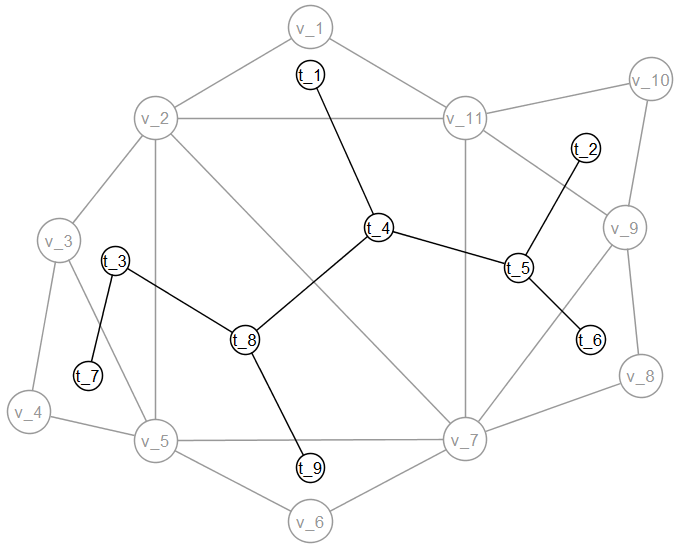
\includegraphics[scale=0.5]{Baumzerlegung.png}
 		\caption{Baumzerlegung}
 		\label{baumzerlegung1a}
 	\end{figure}
 	
 	Figure \ref{baumzerlegung1a} zeigt die gewünschte  Baumzerlegung $(T,\{V_t:t\in T \})$, wobei $T= \{t_i : 1 \le i \le 9\}$ und $V_{t_1}=\{v_1,v_2,v_{11}\}$, $V_{t_2}=\{v_9,v_{10},v_{11}\}$, $V_{t_3}=\{v_2,v_3,v_5\}$, $V_{t_4}=\{v_2,v_{11},v_7\}$, $V_{t_5}=\{v_7,v_9,v_{11}\}$, $V_{t_6}=\{v_7,v_8,v_9\}$, $V_{t_7}=\{v_3,v_4,v_5\}$, $V_{t_8}=\{v_2,v_5,v_7\}$, $V_{t_9}=\{v_5,v_6,v_7\}$ gilt.
 	
	\item Das Ziel des Algorithmus ist es, aus jedem Dreieck in dem Graphen einen Knoten $t \in T$ zu finden, so dass $|V_t| = 3$ gilt. \textbf{Eingabe:} Ein triangulierter Kreisgraph $G=(V,E)$. \\
	Nun betrachten wir zwei Fälle: \\
	\\
	\textit{1. Fall:} Der Eingabegraph $G$ besteht nur aus drei Knoten. In diesem Fall ist $T$ Einelementig und $V_t=V$ für $t\in T$. \\
	\\
	\textit{2. Fall:} Der Eingabegraph $G$ besteht aus mehr als drei Knoten. In diesem Fall werden die äußeren Dreiecke des Graphen $G$ betrachtet. Ein äußeres Dreieck besitzt einen (in diesem Fall genau einen) Knoten $v$ mit Grad = 2. $v$ bildet mit seinen beiden Nachbarknoten ein äußeres Dreieck. Der Algorithmus sucht also in dem Graphen $G$ einen Knoten $v$, dessen Grad = $2$ ist. Für dieses $v$ wird ein Knoten $t$ und die Menge $V_t = {v} \cup {Nachbarn(v)}$ in die Baumzerlegung hinzugefügt. Anschließend wird der Knoten $v$ aus $G$ entfernt und der nächste Knoten mit Grad = $2$ gesucht.     
\end{enumerate}

\section*{Aufgabe 2}

\begin{enumerate}[a)] 
	\item Zunächst sei gezeigt, dass der Algorithmus nur Lösungen überprüft, deren Abstand höchstens $d$ sind. Hier sei darauf zu achten, dass es sich beim Algorithmus um eine rekursive Definition handelt, welche das $d$ in jedem Schritt um $1$ reduziert und gleichzeitig den Abstand von $\Phi$ und $\Phi'$ um $1$ erhöht. Zusammen mit der Abbruchbedingung, dass $d=0$ gilt, betrachtet der Algorithmus nur Lösungen, die einen maximalen Abstand $d$ von der ursprünglichen Belegung $\Phi$ haben. Nun zeigen wir die Behauptung der Aufgabe in beide Richtungen: Wenn der Algorithmus "`yes"' ausgibt, dann gibt es eine erfüllende Belegung $\Phi'$. Diese Richtung ist einfach, da der Algorithmus für eine gegebene Belegung überprüft, ob diese alle Klauseln erfüllt. Nur wenn dies der Fall ist, so wird "`yes"' zurück gegeben. Nun die andere Richtung: Gibt es eine erfüllende Belegung mit maximalem Abstand $d$ um $\Phi$ herum, so wird vom Algorithmus "`yes"' ausgegeben. Wie schon oben erwähnt, wird mit jedem Rekursionsschritt der Abstand von der ursprünglichen Belegung um $1$ erhöht. Ein Rekursionsschritt wird nur dann ausgeführt, wenn mindestens eine Klausel nicht erfüllt ist, ansonsten wird "`yes"' ausgegeben. Da beim Rekusrionsaufruf jede mögliche neue Belegung getestet wird, die die aktuelle Belegung für die zunächst nicht erfüllte Klausel erfüllt, wird jede mögliche erfüllende Belegung in Betracht gezogen. Sollte also eine erfüllende Belegung im Umkreis von einer Distanz von $d$ um die ursprüngliche Belegung liegen, so wird diese dann auch gefunden.
		
		Die Laufzeit des Algorithmus lässt sich aus dem Rekursionsbaum ablesen, denn für jeden Knoten dieses Baumes wird jeweils eine Überprüfung zur Belegung ausgeführt. Die Zeit, die zur Überprüfung der Erfüllbarkeit gebraucht wird, hängt von $n$ ab, da es $n$ verschiedene Klauseln gibt, und wir bezeichnen sie mit $p(n)$. Der Rekursionsbaum hat eine Tiefe von $d+1$, da die Wurzel des Baumes den Abstand $0$ zur Anfangsbelegung hat. In jedem Knoten innerhalb des Baumes wird die Funktion erneut dreimal aufgerufen. Dadurch ergibt sich in jeder Ebene $i$ ($i \in \{0,\dots,d\}$) eine Knotenanzahl von $3^i$, also insgesamt eine Summe von
		$$\sum_{i=0}^d 3^i = \frac{1}{2}(3^{d+1} - 1)$$
		womit wir bei einer Laufzeitschranke von
		$$\mathcal{O}(p(n) \cdot 3^{d})$$
		angekommen sind.
		
		\item Der optimierte Algorithmus wählt eine Belegung $\Phi_1$ fest und das Komplement dieser Belegung, $\Phi_2$, als weiteren Startpunkt des Algorithmus. Somit muss der Algorithmus jeweils Belegungen mit einem Abstand von maximal $d = \frac{n}{2}$ überprüfen. Das Umdrehen der Belegung ist von $n$ abhängig und kann innerhalb des $p(n)$ festgehalten werden. Wir starten den Algorithmus zwei mal, in der $\mathcal{O}$-Notation wird jedoch dieser Faktor nicht auftauchen. Wir erhalten
			$$\mathcal{O}(p(n) \cdot 3^\frac{n}{2}) = \mathcal{O}(p(n) \cdot (\sqrt{3})^{n})$$
			womit die gewünschte Laufzeit erreicht worden ist.
\end{enumerate} 

\end{document}